\documentclass[11pt,dvipdfmx,a4paper]{jsarticle}

\usepackage{amsmath,amssymb}
\usepackage{bm}
\usepackage[dvipdfmx]{graphicx}
\usepackage{physics} % http://mirrors.ibiblio.org/CTAN/macros/latex/contrib/physics/physics.pdf
\usepackage{siunitx} %SI単位を楽に出力
\usepackage{mathtools} %環境の追加
% \usepackage{circuitikz} %電気回路をtex中で書く
% \usepackage{caption} %番号なしキャプションを書く
% \usepackage{cancel} %式中に斜線を入れる
% \usepackage{tensor} %テンソルの添え字を書く
% \usepackage{tikz} %図を書く
% \usepackage{ascmac} %四角い枠の中に文章を書く
% \usepackage{float} %figureで[hbp]オプションを使う
% \usepackage{hyperref}  \usepackage{pxjahyper} %ハイパーリンクをつかう
% \usepackage{tablefootnote} %表中に注釈をいれる
% \usepackage[thicklines]{cancel} %数式中の取り消し線
\usepackage[version=4]{mhchem} %化学式の入力
% \usepackage{pdfpages}
% \usepackage{wrapfig} %文章の回り込み
\usepackage[subrefformat=parens]{subcaption} %(a)図のようにすることができるやつ
\usepackage{here}
\usepackage{mathrsfs} % フォントの追加
\usepackage{url} % url を入れる
\usepackage[margin=15mm]{geometry} %余白の削除
\usepackage{tcolorbox}

\graphicspath{{./image/}}

\begin{document}

%出力したpdfを表紙にするとき
% \includepdf[pages=1,noautoscale=false]{cover.pdf}
% \newpage

%texで表紙を書くとき
\quad\\[35mm]
\centerline{\Huge{\textsf{第 6 回}}}
\quad\\[5mm]
\centerline{\Huge{\textsf{応 用 物 理 学 実 験}}}
\quad\\[5mm]
\begin{table}[h]
	\centering
	\begin{tabular}{| c | c |}
		\hline
		\Huge\textsf{{題目}} & \Huge{\textsf{光吸収}} \rule[-5mm]{0mm}{15mm} \\
		\hline
	\end{tabular}
\end{table}
\quad\\[10mm]
\begin{table}[h]
	\centering
	\begin{tabular}{l l}
		\hline
		\LARGE{\textsf{氏\qquad 名}} & \LARGE{\textsf{: 西原 翔}} \rule[0mm]{0mm}{6mm} \\
		\hline
		\LARGE{\textsf{学  籍  番  号}} & \LARGE{\textsf{: 1522068}} \rule[0mm]{0mm}{6mm} \\
		\LARGE{\textsf{学部学科学年}} & \LARGE{\textsf{: 理学部第一部応用物理学科3年}}\\
		\hline
	\end{tabular}
\end{table}
\quad\\[10mm]
\centerline{\LARGE{\textsf{共同実験者:1522064 中井空弥}}}\\[2mm]
\centerline{\LARGE{\textsf{\qquad\qquad\quad\;\;1522091 宮田祟杜}}}\\[2mm]
\centerline{\LARGE{\textsf{\qquad\qquad\quad\;\;1522095 村山涼矢}}}\\[2mm]
\centerline{\LARGE{\textsf{\qquad\qquad\quad\;\;1522B02 中村洸太}}}\\[2mm]
\quad\\[10mm]
\centerline{\LARGE{\textsf{提出年月日:2024年10月03日}}}\\[2mm]
\centerline{\LARGE{\textsf{実験実施日:2024年09月20日}}}\\[2mm]
\centerline{\LARGE{\textsf{\qquad\qquad\quad\;2024年09月27日}}}
\quad\\[10mm]
\centerline{\LARGE{\textsf{東 京 理 科 大 学 理 学 部 第 1 部}}}\\[2mm]
\centerline{\LARGE{\textsf{応 用 物 理 学 教 室}}}

\thispagestyle{empty}
\clearpage
\addtocounter{page}{-1}
\newpage

\section{目的}
新しい試料を作ったときにまず何を測定するのか。
それはまずサンプルを「見る」ことから始めるものである。
つまり、物質の光学応答の測定こそが物質を調べる基本なのである。

この実験では分光光度計を使い金属(\ce{Au}, \ce{Ag})の光学応答を波長ごとに調べることで、
金属の特徴である金属光沢という光学的性質をスペクトル測定をした。
また、分光は試料の電子構造を知る上で大きな役割を果たしている。
半導体はエネルギーギャップがあるという特徴的な電子構造を持っている。
このエネルギーギャップに由来する光学特性を確認するため、半導体である\ce{SrTi_3}, \ce{CdS}, \ce{GaAs}の光学応答を調べた。

% TODO: DFT の話も入れたいね

\section{原理}
\subsection{光学応答を表すパラメータ}
光学応答を表すパラメータは等価なものとして、(複素)誘電率、(複素)屈折率、反射率・透過率、
の3つがある。

誘電率は光学現象を微視的な観点から説明する際に用いられるものである。
光は電磁場であることが知られているが、磁場による相互作用は電場に比べて弱い。
% 例えば電場と磁場を同じ単位として扱う cgs 系でのローレンツ力の表式は
% \begin{align}
%     F = q \qty(E + \frac{v}{c} B)
% \end{align}
% というように書かれる。荷電粒子の速度\(v\)は光速\(c\)に比べて小さいのでローレンツ力という相互作用では磁場が見えてこない。
なの基本的には光は磁気相互作用のない電場であると考え、そのような電場を光電場と呼ぶ。
光電場\(E\)が媒質中に入ったとき、
媒質中の電荷分布はその光電場によって偏り、分極\(P\)が生じる。
その関係式を\(P = \epsilon_0\chi E\)というように比例するとしたとき、
媒質中での電束密度\(D\)は
\begin{align}
    D = \epsilon_0 E + P = \epsilon_0(1+\chi)E
\end{align}
というように書くことができる。
このとき、電場によって励起された分極\(P\)の影響を誘電率に取り込んで真空と同じように扱う。
つまり、媒質中では誘電率が\(\epsilon=\epsilon_0 (1+\chi)\)の真空であると考える。
この媒質の持つ誘電率というパラメータは実際には相互作用が伝播していく速度が有限であることから、
周波数に依存すると考えると扱いやすい。
このように周波数で誘電率を扱ったものを誘電関数という。

実際には光電場はすべて分極を作るのに使われるのではなく、電流や熱になる。
熱になるのは少なく、電流になるのがほとんどであるのでこれについて考える。
オームの法則により\(j=\sigma E\)と書ける。
時間をフーリエ変換したアンペール・マクスウェルの式にこれらの式を入れると
\begin{align}
    \curl H(\omega) = j(\omega) - i\omega D = -i\omega \qty(\epsilon+\frac{i\sigma}{\omega}) E(\omega)
\end{align}
となる。これを見ると
\begin{align}
    \tilde{\epsilon}(\omega) = \epsilon(\omega) + \frac{i\sigma}{\omega}
\end{align}
として複素数で誘電関数を書くと真空と同じような形
\begin{align}
    \curl H(\omega) = -i\omega \tilde{\epsilon}(\omega) E(\omega)
\end{align}
で書くことができる。
これを複素誘電関数や複素誘電率と呼ぶ。
このように複素誘電率は電場と分極の関係から導かれたものである。
電場と電子の相互作用をモデル化すれば具体的な式の形はわかるものの、
実際の目に見える光学現象との対応がわかりにくく、直接測定することはできない。

これをすこし取り扱いしやすくしたのが屈折率である。
屈折率は媒質中を通る光電場の様子を用いて光学応答を表すものである。
複素誘電率\(\tilde{\epsilon}\)の媒質中では、光の速度は
\begin{align}
    c' = \frac{c}{\sqrt{\tilde{\epsilon}/\epsilon_0}}
\end{align}
と書ける。
これは光学における媒質による光速の違いを表す式
\begin{align}
    c' = \frac{c}{n}
\end{align}
に対応している。ここでの\(n\)は屈折率と呼ばれ光学では実数であるが複素数に拡張してみる。
複素屈折率を
\begin{align}
    \tilde{n} &= n + i\kappa = \sqrt{\tilde{\epsilon}/\epsilon_0}
\end{align}
というように定義する。これを複素屈折率と呼び
複素を付けず単に屈折率といったときには複素屈折率の実部を指し、虚部は消衰係数と呼ばれる。
これらと誘電関数の実部と虚部を\(\epsilon_1=\Re(\tilde{\epsilon}/\epsilon_0),\,\epsilon_2=\Im(\tilde{\epsilon}/\epsilon_0)\)の間には
\begin{align}
    n^2-\kappa^2 = \epsilon_1,\qquad 2n\kappa = \epsilon_2
\end{align}
という対応関係がある
これを使うと複素屈折率\(\tilde{n}\)の媒質中を通る光を次のよう表せる。
\begin{align}
    E &= E_0 e^{-i\omega (t - \tilde{n}x/c)} = E_0 e^{-\omega \kappa x / c}e^{-i\omega (t - x/(c/n))}
\end{align}
この表式よりに媒質中を通る光の速度とその減衰の様子を表してるのがわかる。
波動現象によってはこの量は測定しやすい。
光においてはこの量は干渉計や光の強度を測定することで求めることができるものの、
これでもまだ煩雑である。

より直接的に測定できる量は反射率と透過率である。
2つの媒質の境界面に入射する光の強度を\(\abs{E_i}^2\),
その面で反射する光の強度を\(\abs{E_r}^2\),
その面を透過する光の強度を\(\abs{E_t}^2\)
としたときに、反射率 \(R\) と透過率 \(T\) は
\begin{align}
    R = \frac{\abs{E_r}^2}{\abs{E_i}^2},\qquad  T = \frac{\abs{E_t}^2}{\abs{E_i}^2}
\end{align}
というようにあらわされる量である。
この量は試料を反射した光との強度を測定することで得られる量である。
そのため直感的にわかりやすく、測定もしやすい量である。

反射率・透過率、複素屈折率は電場の境界面における境界条件を計算すると結びつけられる。
複素屈折率が\(\tilde{n}_1\)の媒質から複素屈折率が\(\tilde{n}_2\)の媒質へ垂直に入射するときには
\begin{align}
    t = \frac{2\tilde{n}_1}{\tilde{n}_1 + \tilde{n}_2},\qquad  r = \frac{\tilde{n}_2-\tilde{n}_1}{\tilde{n}_1+\tilde{n}_2}
\end{align}
という量を用意すると
この面での反射光と透過光は
\begin{align}
    E_{r1} = r_1 E_i, \qquad E_{t1} = t_1 E_i
\end{align}
と書ける(p偏光におけるフレネルの式)。
このとき光のエネルギーについてポインティングベクトルを考慮すると、
反射光は入射光と同じ媒質を伝播するので単に
\begin{align}
    R = \abs{r}^2 = \abs{\frac{\tilde{n}_2-\tilde{n}_1}{\tilde{n}_1+\tilde{n}_2}}^2
\end{align}
というように対応づけることができる。
透過光は伝播する速度が入射光・反射光と違うため\(T\neq\abs{t}^2\)であり、
\begin{align}
    T &= 1 - R = \frac{2(\tilde{n}_1^*\tilde{n}_2+\tilde{n}_1\tilde{n}_2^*)}{\abs{\tilde{n}_1+\tilde{n}_2}^2}
\end{align}
となる。
とくに、\(\tilde{n}_1=1, \tilde{n}_2 = \tilde{n}\)のときには
\begin{align}
    R & = \abs{\frac{1-\tilde{n}}{1+\tilde{n}}}^2\\
    T & = \frac{4n}{\abs{1+\tilde{n}}^2}
\end{align}
と書ける。
光が透過するときには実際の試料では光が入射する面と出ていく2つの面があり、
この2つの面の間で多重反射した光が透過光強度として測定される。
試料の面の法線方向から\(\theta\)だけ傾いた方向から光が入射したとして、
試料の厚さを\(d\), 吸収係数と呼ばれる量を\(\alpha=2\omega\kappa/c\)を使うと、このときの透過率\(T'\)と反射率\(R'\)は
\begin{align}
    T' &= \frac{(1-R^2)\exp(-\alpha d\cos\theta)}{1-R^2\exp(-2\alpha d\cos\theta)}\\
    R' &= R(1+T'\exp(-\alpha d\cos\theta))
\end{align}
となる。実際に測定される透過率・反射率は試料自身の誘電関数から得られる方ではなくこの量である。
この式を\(\alpha d \cos\theta\)と\(R\)について解くと
\begin{align}
    \alpha d  \cos\theta&= \arcsin(\frac{(1-R')^2-T'^2}{2T'})\\
    R &= \frac{R'}{1+T'\exp(-\alpha d cos\theta)}
\end{align}

以上より誘電関数と反射率・透過率がきちんと対応することが分かった。
実験から反射率と透過率を測定し、それを説明するような誘電関数を導くモデルが作れたのなら、
それが光学現象の機構であると考えれるのがわかる。

\section{実験}
タングステンランプと重水素ランプを用いた分光光度計である Hitach U-3900 を用いて
金属(\ce{Au}, \ce{Ag})と半導体(\ce{GaAs}, ウルツ鉱型\ce{CdS}, \ce{SrTiO_3})の反射率測定を 200nm - 1050nm の領域で行った。
また半導体試料については透過率測定も同様に 200nm - 1000nm の領域で行った。透過率測定を行った試料の厚さは 0.5 mm であった。

\section{結果}
試料の反射率の測定結果は図\ref{graph:01}のようになった。
金属試料である\ce{Au}と\ce{Ag}、半導体試料である\ce{GaAs}, \ce{CdS}, \ce{SrTiO_3} では反射率の振る舞いが違うのがわかる。
金属試料は高エネルギーでは反射率が低く、ある波長よりも低エネルギーになると反射率が高くなっているのに対し、
半導体試料では反射率は金属試料試料ほどの大きな変化はしていない。
金属のこの波長に対応する光の振動数はプラズマ振動数と呼ばれている。
高エネルギーになると反射率は大きくなっている。
また、反射率の波長依存性は試料がどのように見えるかに直接かかわってくる(課題3).
反射率が大きい波長の光は見え、低いところの波長は見えない。
図\ref{graph:01}の結果より、金は緑色から青色の光はなく、
赤色から緑色の光が重ね合わさった色が見える。
つまり黄色の物質として見えるというのこのスペクトルからわかる。
残りの試料については課題のセクションで言及する。

試料の透過率の測定結果は図\ref{graph:02}のようになった。
ある波長より高エネルギーになると透過率が 0 になり試料が光を通さなくなることがわかる。
この波長を反射率の方でも確認すると反射率の値が階段状になっているのに気付く。
これは半導体のバンドギャップに由来する振る舞いであると理解され、
この波長に対応する光子エネルギーが半導体のエネルギーギャップである。
これよりエネルギーギャップは \ce{SrTiO_3} が 3.23 eV, CdS が 2.38 eV, GaAs が 1.40 eV であるのがわかる。

\begin{figure}[H]
    % \centering
    \begin{minipage}[t]{0.48\columnwidth}
        \centering
        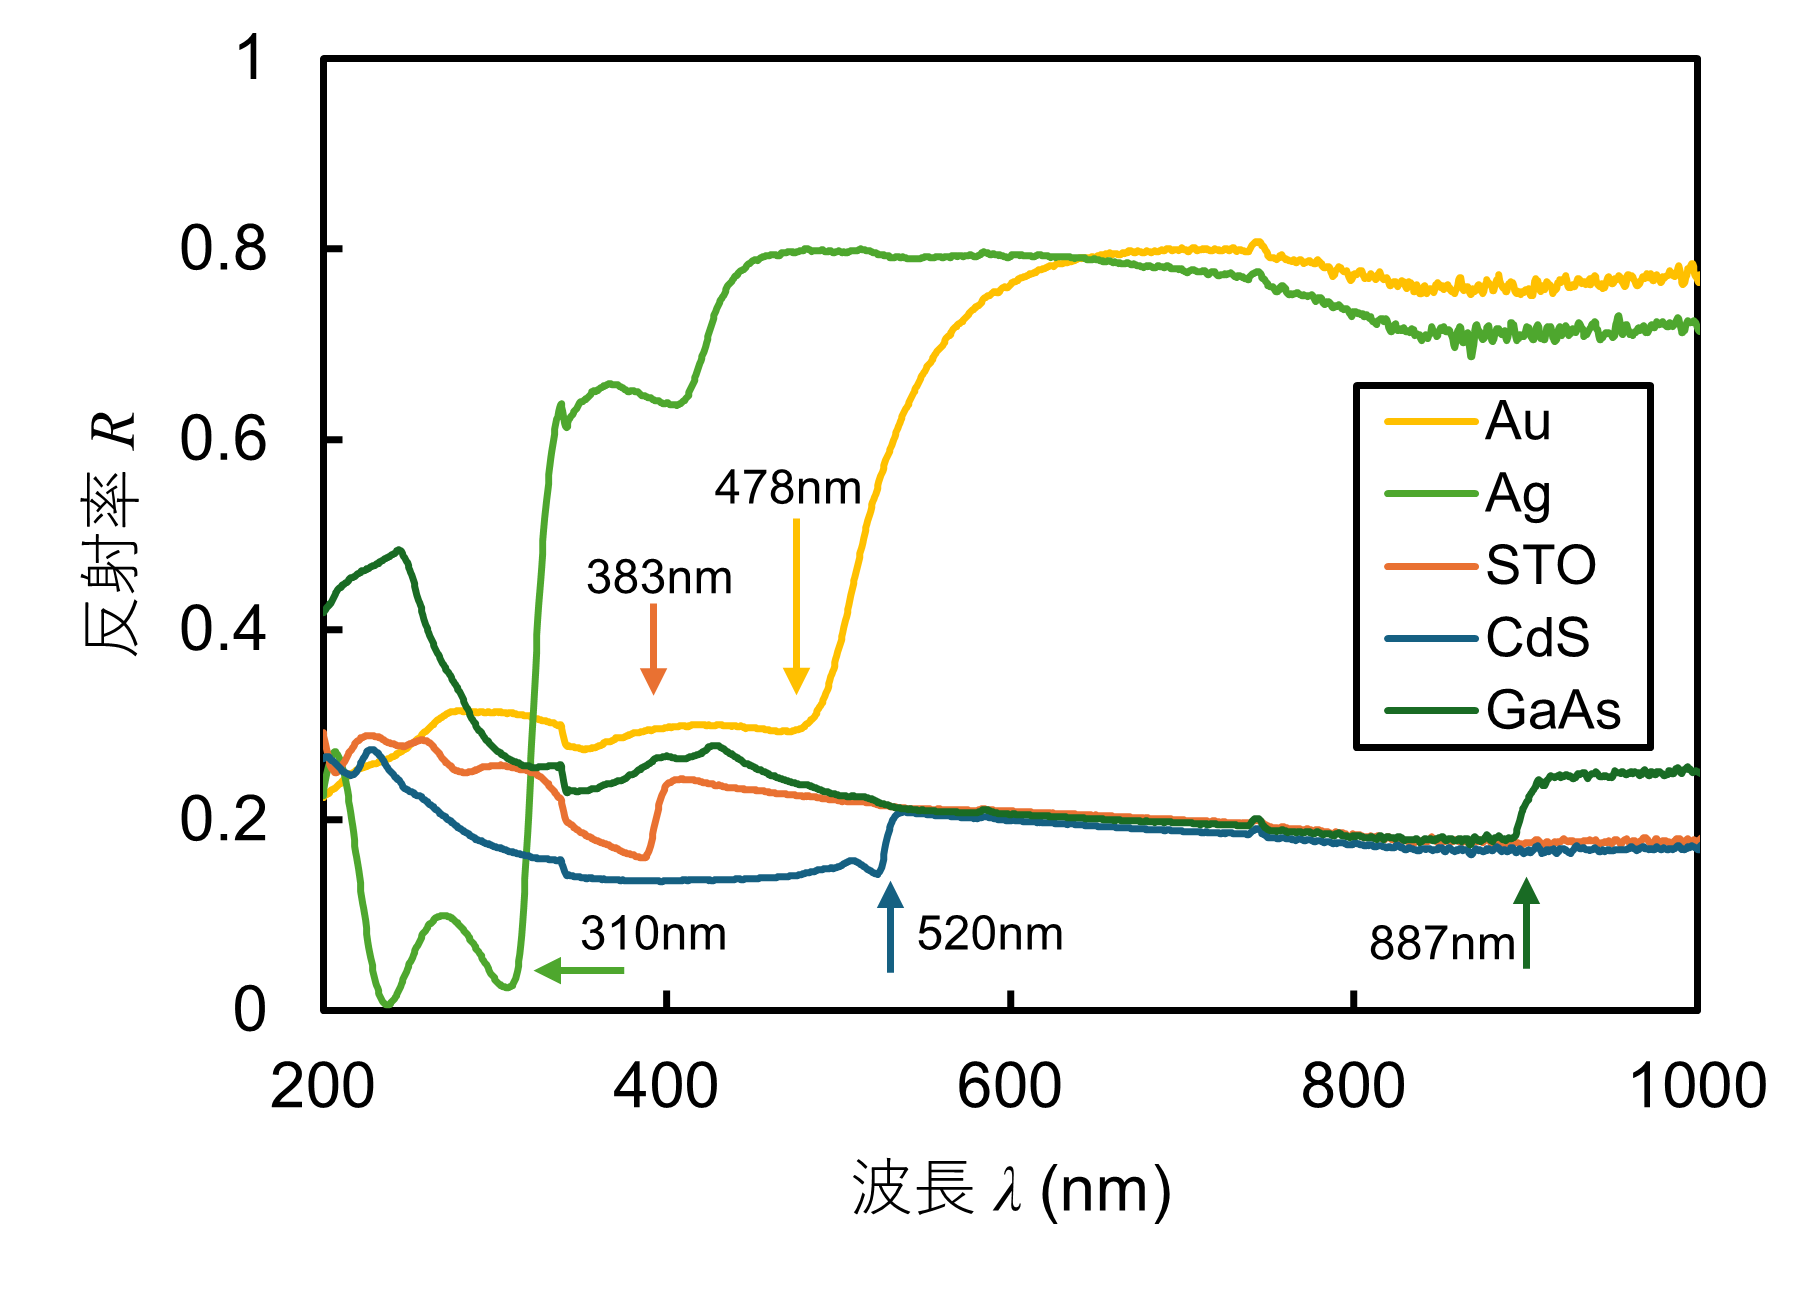
\includegraphics[width = \columnwidth]{graph/graph1.png}
        \caption{金属(\ce{Au}, \ce{Ag})と半導体(\ce{GaAs}, ウルツ鉱型\ce{CdS}, \ce{SrTiO_3})の反射率の測定結果。
        金属はプラズマ振動数、半導体はエネルギーギャップに対応する波長が書き込んである。}
        \label{graph:01}
    \end{minipage}
    \hfil
    \begin{minipage}[t]{0.48\columnwidth}
        \centering
        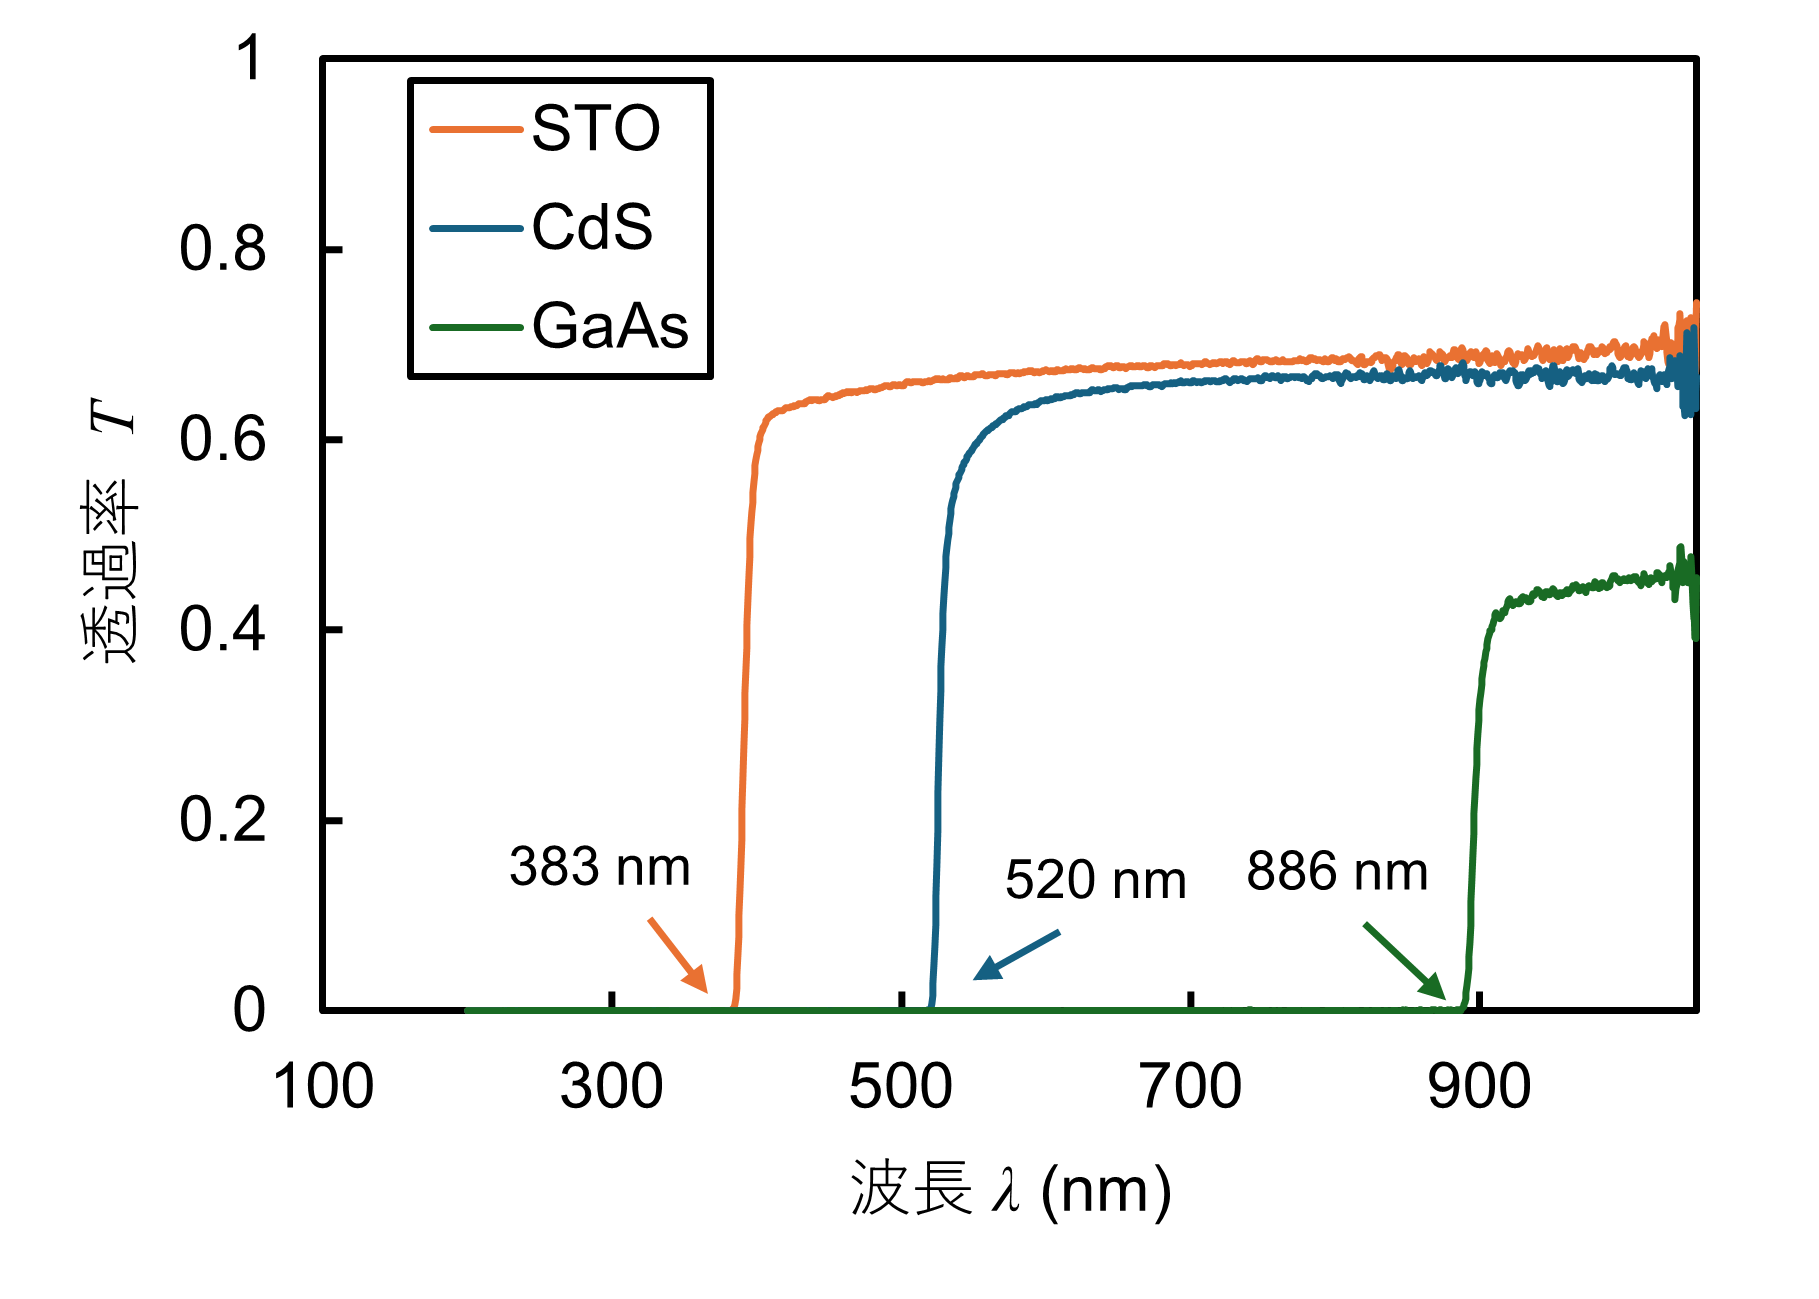
\includegraphics[width = \columnwidth]{graph/graph2.png}
        \caption{半導体(\ce{GaAs}, ウルツ鉱型\ce{CdS}, \ce{SrTiO_3})の反射率の測定結果。
        エネルギーギャップに相当する波長で透過率が大きく変化している。}
        \label{graph:02}
    \end{minipage}
\end{figure}

\section{考察}
反射率と透過率の測定結果を他のパラメータに読み替えて結果を分析していく。
(19)式と(20)を使って半導体試料の測定した反射率・透過率から吸収係数\(\alpha\)を求めると図\ref{graph:03}のようになった。
測定装置の測定できる強度の精度は\(1.0\times10^{-5}\)までである。
これよりより小さい値は測定データとしては非正の値となるため、
計算の都合上\(1.0\times10^{-5}\)であるとして処理をした。
いづれも透過率が大きく変化した波長において吸収係数が大きく変化しているのがわかる。
半導体のエネルギーギャップ付近吸収係数の変化の仕方に注目すると、
\ce{SrTiO_3} と CdS, GaAs で違うのがわかる。\ce{SrTiO_3} では対数プロットで傾きがあるのがわかるのに対して、
CdS, GaAs ではほとんど垂直に変化している。
これは半導体のエネルギーギャップでの電子の励起が直接遷移型であるか、間接遷移型であるかで説明される。
\ce{CdS}と\ce{GaAs}のバンド図を Quantum espresso という第一原理計算のソフトを使ってバンド図を計算すると、
図\ref{band}のようになった。\footnote{どんなパラメータのもと、どんな疑ポテンシャルを使ったのかは割愛する。}
これを見ると波数空間の原点である\(\Gamma\)にて直接遷移が起きるのがわかる。
またこのバンド図よりエネルギーが\ce{CdS}では 2.3 eV, \ce{GaAs}では 1.4 eV であるのも読み取れる。
この値が小さく出るのは第一原理計算の仕組み上不可避である。\cite{DFT}
\begin{figure}[H]
    \begin{minipage}[t]{0.48\columnwidth}
    \centering
    % 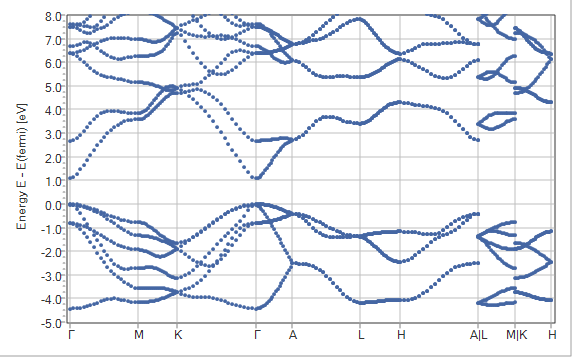
\includegraphics[width = \columnwidth]{band/CdS.png}
    \subcaption{CdS}
    \end{minipage}
    \hfil
    \begin{minipage}[t]{0.48\columnwidth}
        \centering
        % 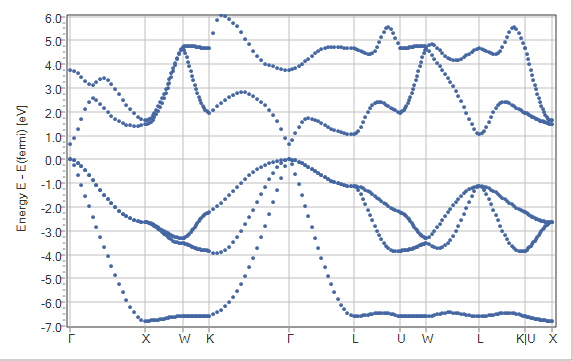
\includegraphics[width = \columnwidth]{band/GaAs.png}
        \subcaption{GaAs}
    \end{minipage}
    \caption{Quantum espresso で計算した直接遷移型の半導体のバンド図}
    \label{band}
\end{figure}
エネルギーギャップの大きさを\(E_g\), 間接遷移にかかわる格子振動との散乱のエネルギーを\(\hbar\Omega\)としする。
光のエネルギーが\(\hbar\omega \gtrsim E_g\)では吸収係数\(\alpha\)は
直接遷移において
\begin{align}
    \alpha \propto \frac{\sqrt{\hbar\omega -E_g}}{\hbar \omega}
\end{align}
間接遷移おいて
\begin{align}
    \alpha \propto \frac{1}{\hbar\omega}\qty[
        \frac{(\hbar\omega+\hbar\Omega -E_g)^2}{e^{\beta\hbar\omega}-1}
        + \frac{(\hbar\omega-\hbar\Omega -E_g)^2}{e^{-\beta\hbar\omega}-1}
    ]
\end{align}
になることがブロッホ電子について、周期的な外場のある摂動論を計算するとわかる\cite{mikoshiba}。
これの\(\hbar\omega \gtrsim E_g\)での傾きを考えると、
直接遷移の傾きは\(1/(\hbar\omega-E_g)\),
間接遷移での傾きは 0 となる。
吸収係数の測定結果(図\ref{graph:03})のエネルギーギャップでの振る舞いの違いは確かに表れるのがわかる。
これを踏まえてこれらの関数でフィッティングすると図\ref{graph:05}のようになる。\footnote{\ce{SrTiO_3}のフィッティングは間に合いませんでした。}
結果としては実験中に指示された直線によるフィッティングと同じことをやっているが、
バンドギャップ付近だけではなくより高エネルギーにおいても使えるものになっている。

\begin{figure}[H]
        \begin{minipage}[t]{0.48\columnwidth}
        \centering
        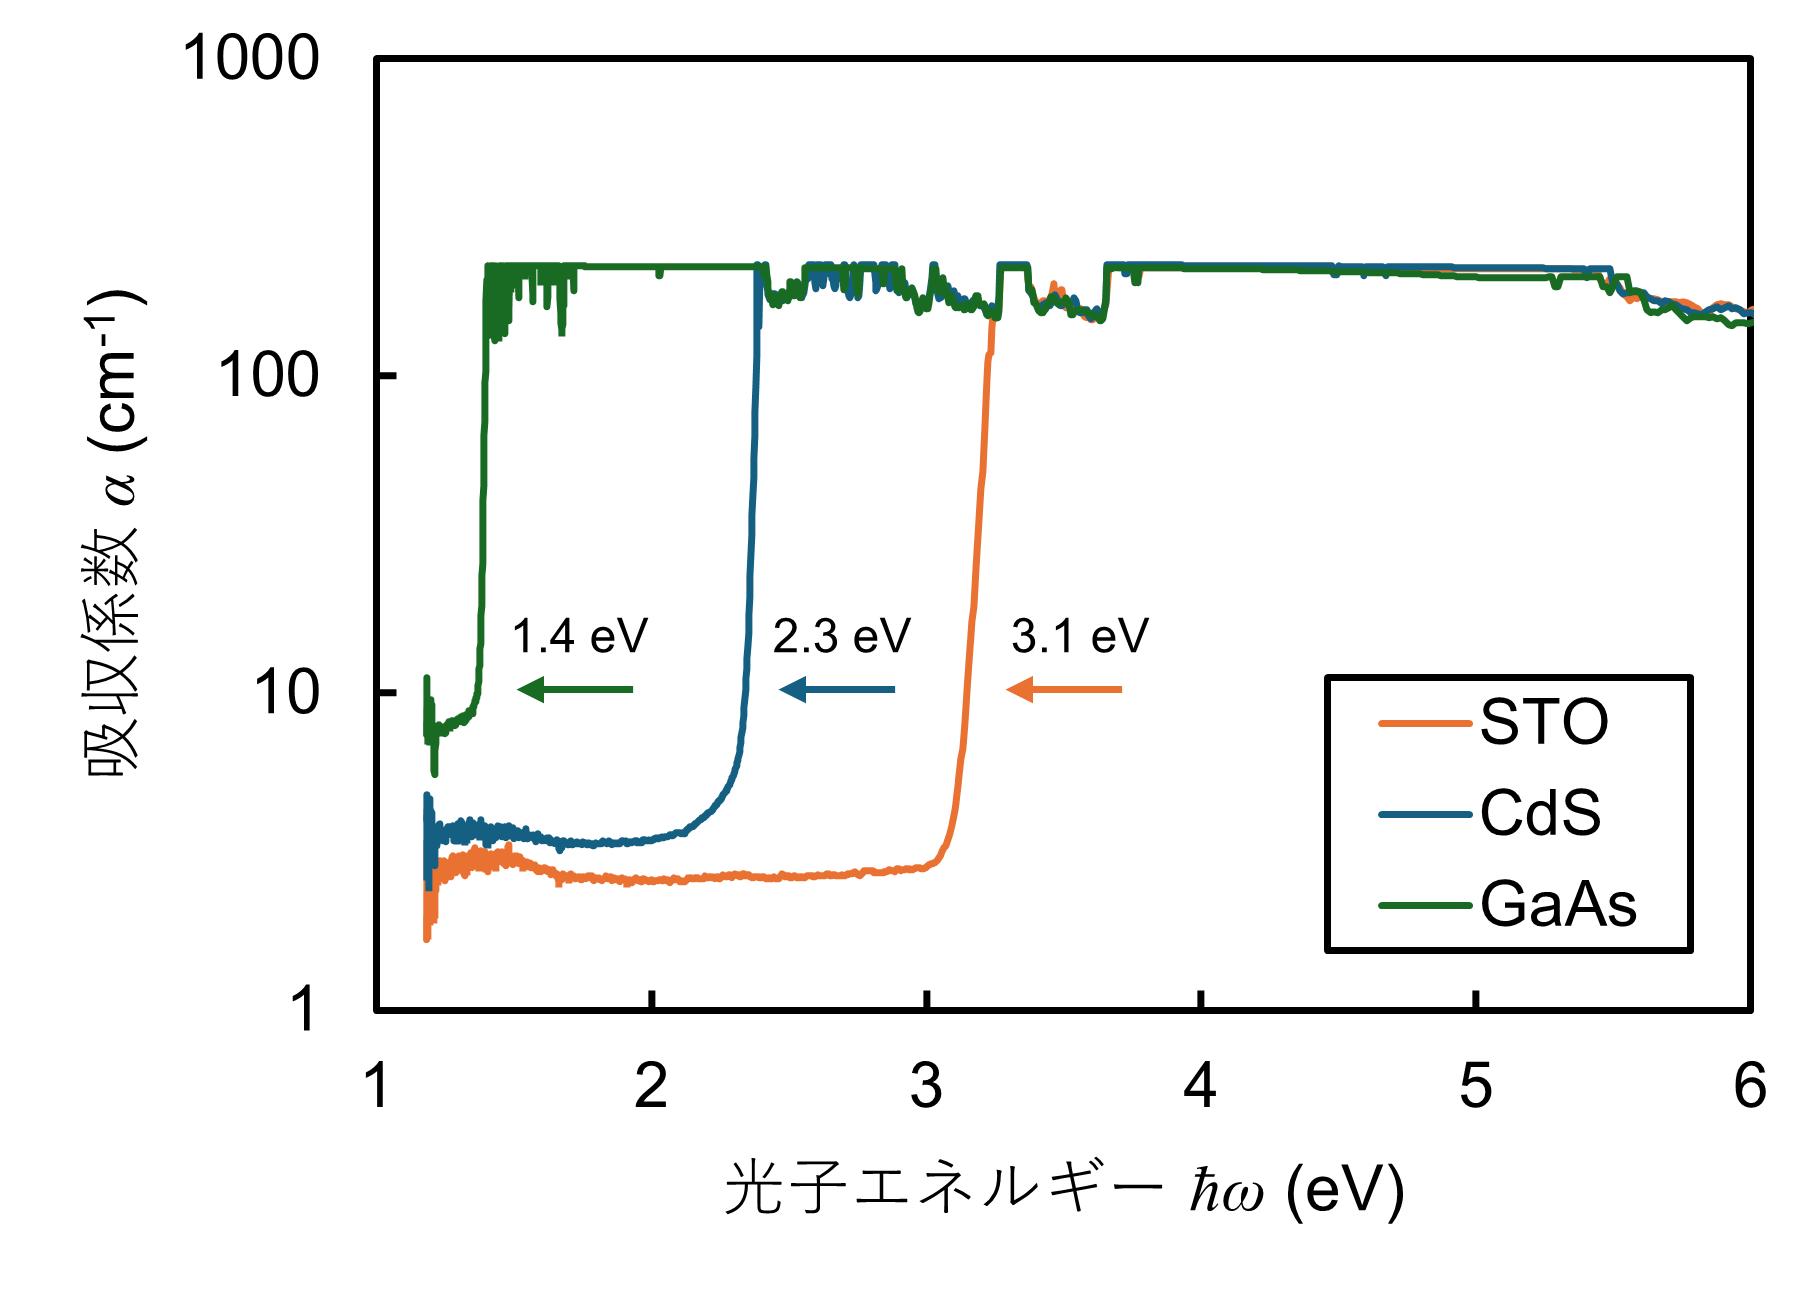
\includegraphics[width = \columnwidth]{graph/graph3.png}
        \caption{半導体(\ce{GaAs}, ウルツ鉱型\ce{CdS}, \ce{SrTiO_3})の各波長における吸収係数}
        \label{graph:03}
    \end{minipage}
    \hfil
    \begin{minipage}[t]{0.48\columnwidth}
        \centering
        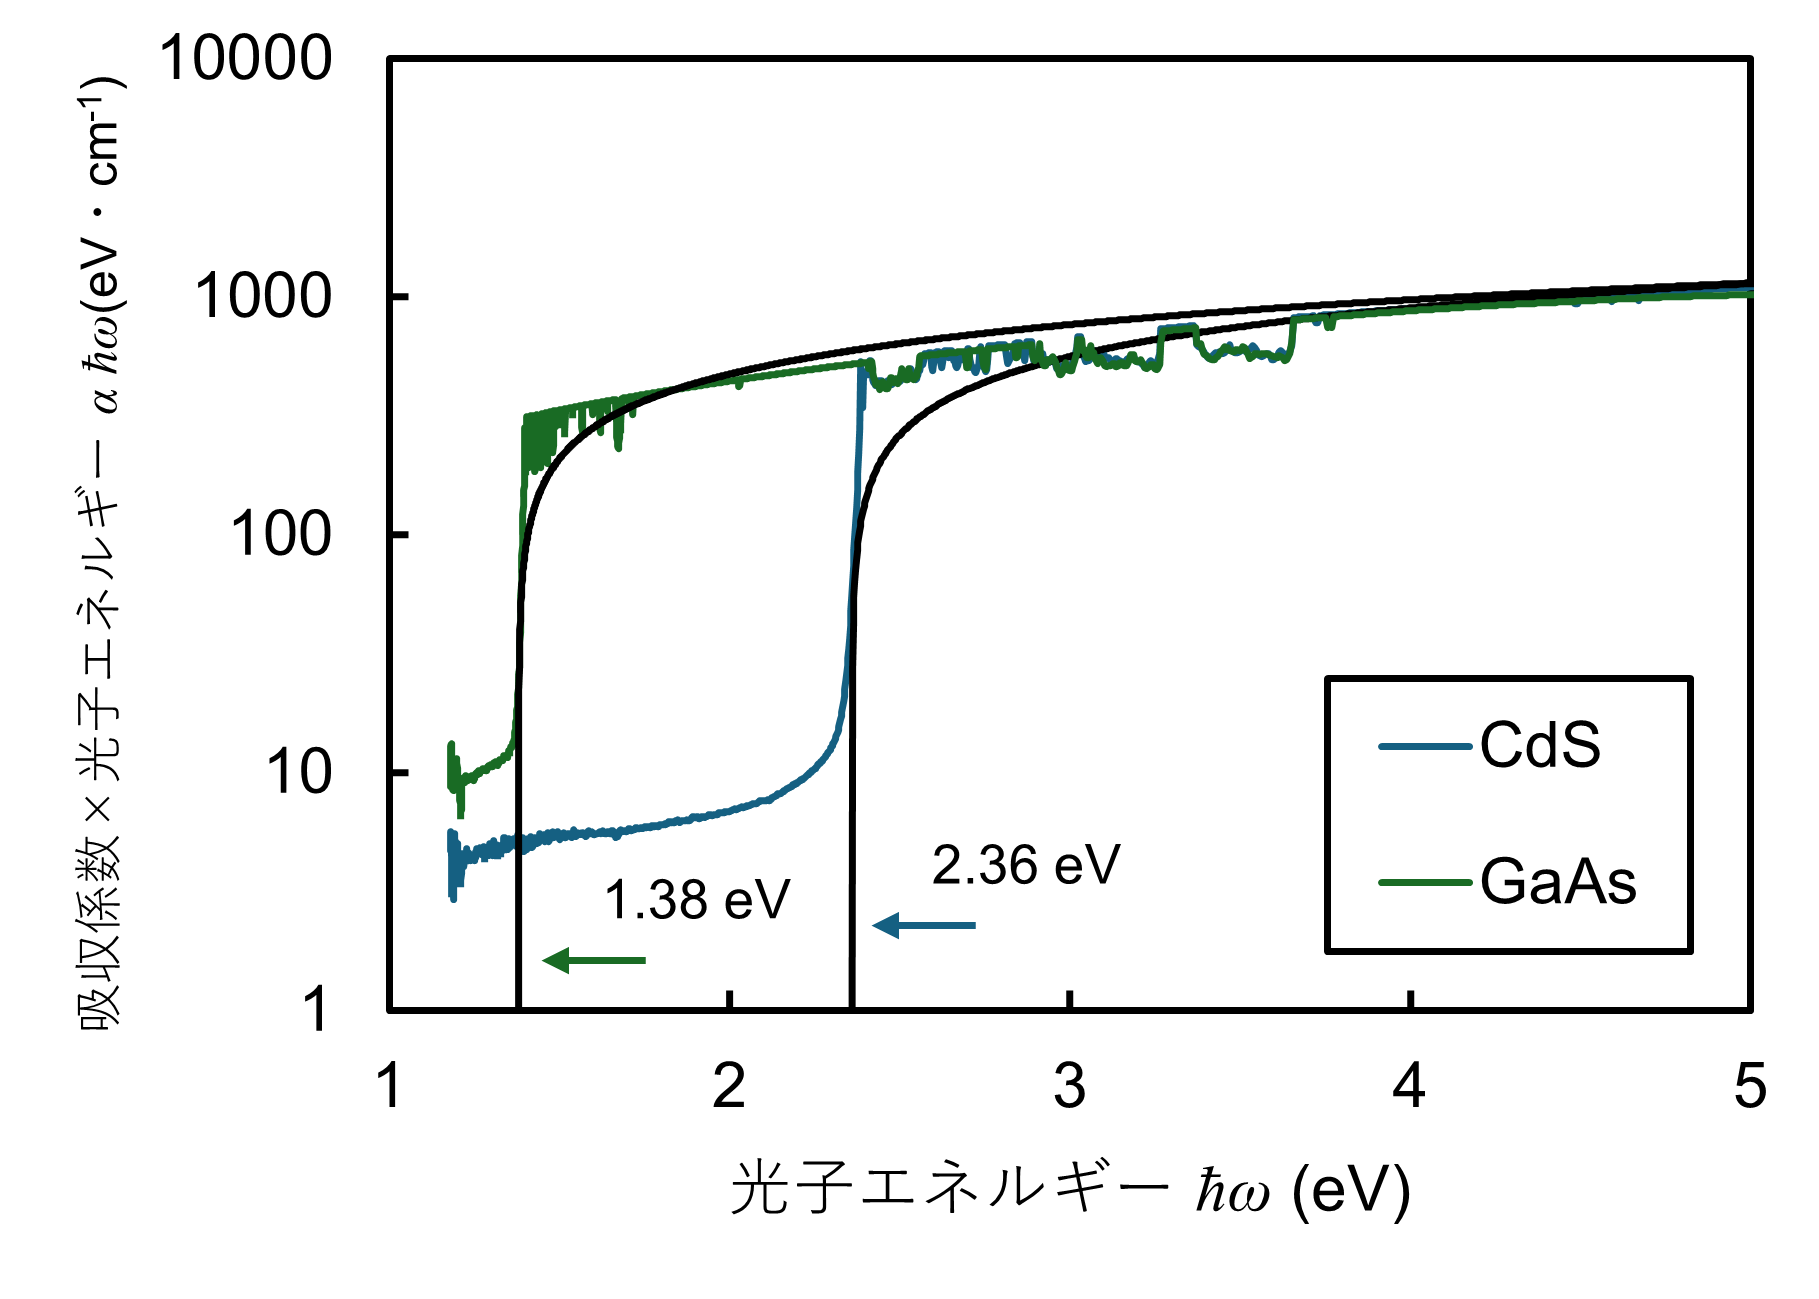
\includegraphics[width = \columnwidth]{graph/graph5.png}
        \caption{直接遷移型半導体\ce{GaAs}, ウルツ鉱型\ce{CdS}, \ce{SrTiO_3}の吸収係数を(21)式を使ってフィッティングしたグラフ}
        \label{graph:05}
    \end{minipage}
\end{figure}

\section{課題}
\begin{tcolorbox}[title = 課題1]
    マニュアルを参考にし、
    使用した分光系である Hitachi U-3900 の仕組みを記述せよ。
    特に、リファレンス側とサンプル側に分かれている意義、
    ベースライン測定をする意義、
    波長を変えた測定をするしくみ、
    についてわかりやすく述べよ。
    また、実験条件である波長範囲、スリット幅、サンプリング間隔、スキャンスピード
    を決定する際に留意すべき点を記述せよ。
\end{tcolorbox}

\begin{tcolorbox}[title = 課題2]
    金および銀について、
    反射スペクトルが大きく変化する振動数によりプラズマ振動数を推定せよ。
    また金属中の電子を自由粒子であるとするドルーデモデルを仮定したときのプラズマ振動数の理論値を計算せよ。
    さらに推定値と理論値に差が生じる理由を物理的に考察せよ。
\end{tcolorbox}

\begin{tcolorbox}[title = 課題3]
    今回測定した試料の反射率スペクトルと透過率スペクトルから、
    各試料の色について考察せよ。
\end{tcolorbox}

反射率に波長依存性があるということは
反射率が大きい波長の光は見え、低いところの波長は見えないということである。
すると白色光を当てて試料を眺めたときに、
目に見えるのは特定の波長をもった色の光であるので、
試料には特有の色があると認知する。
また透過率が高いと試料を通して後ろの様子が透けて見える。
波長によって透過率が違うということは特定の色の光だけが見えるということである。
色のついたフィルムというのは透過率の言葉で言うと、
特定の波長をもった光だけを透過しているというものである。
それを踏まえて今回測定した試料である \ce{Au}, \ce{Ag}, \ce{SrTiO_3}, \ce{CdS}, \ce{GaAs}
の反射率スペクトルと透過率スペクトルと実際の見え方を比べる。

図\ref{graph:01}の結果より、\ce{Au}は緑色から青色の光は弱く、
赤色から緑色が強い光の色が見える。
つまり黄色の物質として見えるというのがこのスペクトルからわかる。
これは実際の経験と合っている。

\ce{Au}は可視光の範囲ではどの波長の光も同じ程度の強さで反射することから、
白色光を入れたとき同じく白色が見えるような白色の金属であるというのがスペクトルからわかる。
これは実際の経験と合っている。

\ce{SrTi_3}と\ce{CdS}は可視光の範囲ではほとんど一定で互いに同じ反射率となっているので白色をした見た目であるとスペクトルからわかる。
\ce{GaAs} はバンドギャップに対応する波長である 520 nm で反射率が少し変化しているので、少しだけ黄色に見える。

また図\ref{graph:02}の透過率について注目すると
\ce{SrTiO_3}は可視光の範囲では常に光を透過するのがわかる。
このスペクトルより\ce{SrTiO_3}は少し暗い透明な物質であると人の目には認識される。
透明な半導体であることを利用したデバイスというのも世の中には多くあるのだろう。

\ce{CdS} は緑の光より高エネルギーの光を通さないものであるというのがわかる。
つまりこれは緑色のレーザーポインタを当てたときに透過することはないが、
赤色のレーザーポインタを当てると透過することを表す。
このことからきれいな単結晶を用意すればレーザーポインタを \ce{CdS} にあてるだけで、
結晶の回折を見ることができ、回折パターンから結晶構造が推定できることが予想される。

\ce{GaAs} は可視光の範囲では光を通さない物質であるのがわかる。
しかし、赤外線は通すので赤外線カメラや赤外線レーザーにとっては\ce{GaAs}は透明であるとみなすことができる。
そして、金属の反射率は 0.8 程度と大きいため明るい色を持った光沢として見えるのに対し、
\ce{GaAs} の反射率は 0.2 程度と金属と比べると小さい。
そのためくすんだ光沢をもった白色として見えるのがわかる。

\section{結論}


\bibliographystyle{junsrt}
\bibliography{reference}
\section*{付録}

\end{document}